% ================================================================
%  Part 4(b) -- Value error versus iteration
%  Required packages (add to your preamble if not already there):
%    \usepackage{amsmath,amssymb,booktabs,graphicx,float}
%  Upload part4b_value_error.png to your Overleaf project.
% ================================================================
\documentclass[11pt]{article}
\usepackage[margin=1in]{geometry}
\usepackage{amsmath,amssymb,booktabs,graphicx,float}
\begin{document}

% ----------------------- copy from here -----------------------
\subsection*{Part 4(b): Value error versus iteration}

\paragraph{Error measure.}
Backward DP (Part~1) gives the exact optimal cost-to-go $J_{\mathrm{DP}}$ on every
augmented state. It is therefore used as the reference, and the error of any value
table $J$ is measured in the sup-norm over all states and stages,
\begin{equation}
  \varepsilon(J) \;=\; \lVert J - J_{\mathrm{DP}} \rVert_\infty
  \;=\; \max_{z \in \mathcal{Z}} \bigl| J(z) - J_{\mathrm{DP}}(z) \bigr| ,
\end{equation}
where $\mathcal{Z}$ contains the $3185$ states $z=(k,e,\eta)$, $k=0,\dots,12$, together
with the absorbing state $\Delta$. For value iteration (VI) the error is recorded after
every synchronous sweep $J_{s}=TJ_{s-1}$. For policy iteration (PI) it is recorded
after every exact policy evaluation, i.e.\ $\varepsilon(J_{\mu_i})$ for the policy
$\mu_i$ of round $i$.

\paragraph{Results.}
Table~\ref{tab:err} and Figure~\ref{fig:err} show the error history. Exact zeros
cannot be drawn on a logarithmic axis, so they are plotted at $10^{-16}$.

\begin{table}[H]
\centering
\small
\begin{tabular}{l*{7}{c}}
\toprule
Iteration & 1 & 2 & 3 & 4 & 5 & 6 & 7 \\
\midrule
VI & 8830 & 7530 & 6090 & 4680 & 3420 & 2360 & 1810 \\
PI & 1850 & 18.2 & 8.13 & 0.852 & \textbf{0} & -- & -- \\
\midrule
Iteration & 8 & 9 & 10 & 11 & 12 & 13 & 14 \\
\midrule
VI & 1340 & 939 & 432 & 124 & 12.5 & \textbf{0} & 0 \\
\bottomrule
\end{tabular}
\caption{Maximum value error $\lVert J - J_{\mathrm{DP}}\rVert_\infty$ after each VI
sweep and after each PI policy evaluation.}
\label{tab:err}
\end{table}

\begin{figure}[H]
\centering
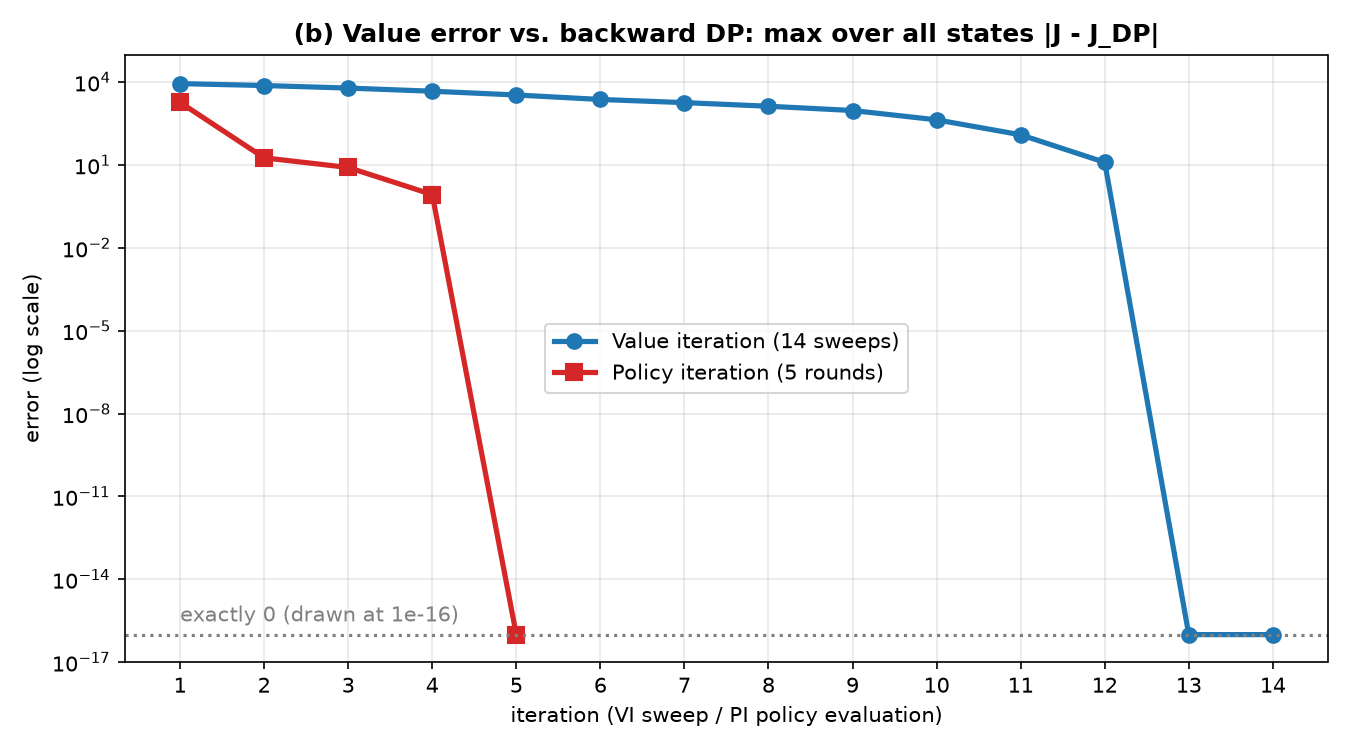
\includegraphics[width=0.85\linewidth]{part4b_value_error.png}
\caption{Value error relative to backward DP versus iteration (logarithmic scale).
VI: error after each sweep. PI: error after each policy evaluation.}
\label{fig:err}
\end{figure}

\paragraph{Interpretation of the VI curve.}
Starting from $J_0 \equiv 0$, sweep~1 makes layer $k=12$ exact ($J=g_N$), and sweep
$s$ makes layers $k=13-s,\dots,12$ exact, since each layer is computed from the
already exact layer behind it. The error is a maximum over \emph{all} states, so it
stays large until the last layer $k=0$ is exact. This happens at sweep~13, where the
error becomes exactly $0$; sweep~14 only confirms $TJ=J$ (Bellman residual $0<10^{-10}$).
Because $J_0\equiv 0$ and all costs are nonnegative, VI approaches $J^*$ from
\emph{below}: its early values account for only the last few stages of cost.
For example, after sweep~1 the state $(9,-33,-2)$ has value
$33^2+0.25\cdot 4+0.5=1090.5$, while $J^*(9,-33,-2)=9919.99$, which gives the error
$\approx 8830$.

\paragraph{Interpretation of the PI curve.}
Each PI value table is the exact cost of a feasible policy, so
$J_{\mu_i} \ge J^*$ and PI approaches $J^*$ from \emph{above}. The initial policy
$u=-\operatorname{sign}(\eta)$ reacts only to the drift and ignores the reference,
so its error is largest where a position correction is needed but no drift exists,
e.g.\ $J_{\mu_1}(3,15,0)=4366.4$ versus $J^*(3,15,0)=2517.35$ (error $\approx 1850$).
By the policy improvement theorem, $J_{\mu_{i+1}} \le J_{\mu_i}$ at every state, and
the error drops sharply ($1850 \to 18.2 \to 8.13 \to 0.852 \to 0$). It reaches zero
after the fifth evaluation, when no control changes.

\paragraph{Why fewer iterations does not imply less computation.}
PI needs 5 iterations and VI needs 14, but an iteration is not a fixed unit of work.
Let one $Q$-evaluation denote the basic operation
$Q(z,u)=g(e,\eta,u)+\sum_{w}p(w)\,J(k+1,e+\eta-\Delta r_k,\eta+u+w)$.
Since $|\mathcal{U}(\eta)|=1,2,3,2,1$ for $\eta=-2,\dots,2$, a full Bellman backup over
the $552\cdot 5=2760$ decision states ($k\le 11$) costs $9\cdot 552=4968$
$Q$-evaluations. A policy evaluation uses only the fixed control and costs $2760$.

\begin{table}[H]
\centering
\small
\begin{tabular}{lcccc}
\toprule
Method & Work per iteration & Iterations & Total $Q$-evaluations & Time (ms)$^\dagger$ \\
\midrule
Backward DP & $4968$ & 1 & $4{,}968$ & 26.1 \\
Value iteration & $4968$ & 14 & $69{,}552$ & 237.2 \\
Policy iteration & $2760+4968=7728$ & 5 & $38{,}640$ & 89.6 \\
\bottomrule
\end{tabular}
\caption{Computational work. $^\dagger$Median of 7 runs, plotting excluded;
absolute times are machine dependent.}
\label{tab:work}
\end{table}

Three observations follow.
\begin{enumerate}
  \item \textbf{Iterations have different costs.} One PI round (evaluation plus
        improvement) costs $7728/4968 \approx 1.6$ VI sweeps, so the 5 PI rounds
        correspond to about $7.8$ sweeps of work, not 5. PI still wins here, but by
        a much smaller factor than $14/5$ suggests.
  \item \textbf{Exploiting structure matters most.} Backward DP uses the finite-horizon
        ordering directly and computes each layer exactly once. With a single
        iteration it does about $14\times$ less work than VI and $8\times$ less than PI.
        The measured times follow the same ranking.
  \item \textbf{Evaluation can be expensive in general.} Here exact policy evaluation is
        one backward pass because the horizon is finite. For infinite-horizon
        (e.g.\ discounted) problems, exact evaluation requires solving a linear
        system $J_\mu = g_\mu + \alpha P_\mu J_\mu$ with one unknown per state, which
        costs $O(n^3)$ for $n$ states. A single PI iteration may then be far more
        expensive than many VI sweeps.
\end{enumerate}
Hence the iteration count alone is not a measure of computational cost; the fair
comparison is total work, i.e.\ (number of iterations) $\times$ (cost per iteration),
or measured run time.
% ------------------------ copy to here ------------------------

\end{document}
